\documentclass{standalone}
\usepackage{tikz}
\usetikzlibrary{patterns, positioning}
\usepackage[sfdefault]{ClearSans} %% option 'sfdefault' activates Clear Sans as the default text font
\usepackage[T1]{fontenc}

\begin{document}
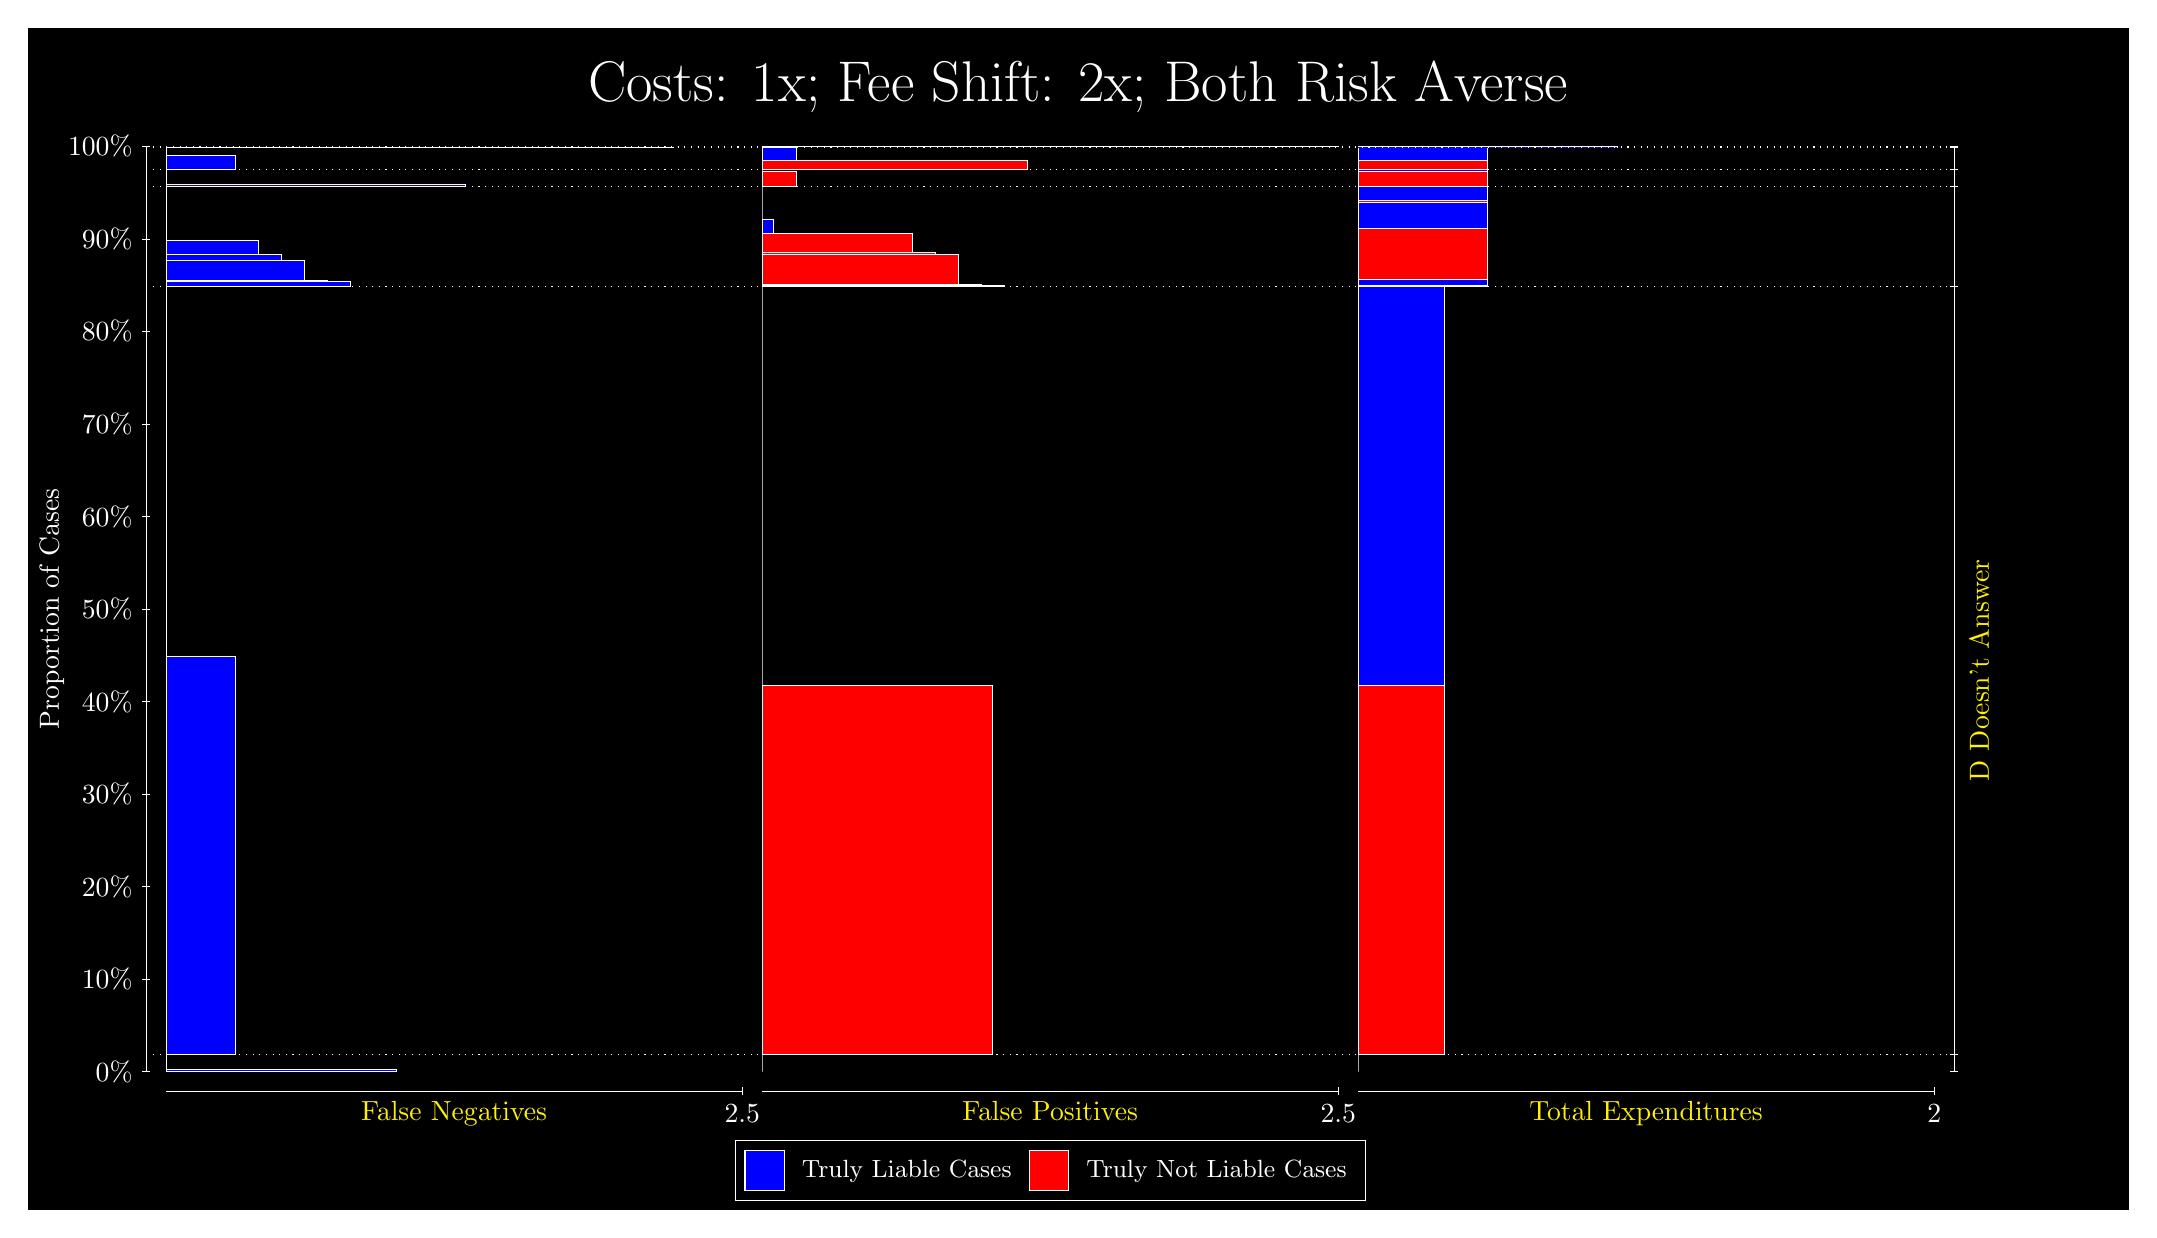
\begin{tikzpicture}
\draw[fill=black] (0,0) rectangle (26.667,15);
\draw[text=white] (0,13.5) rectangle (26.667,15) node[midway] {\huge Costs: 1x; Fee Shift: 2x; Both Risk Averse};
\draw[white, very thin] (1.5,1.75) -- (1.5,13.5);
\node[rotate=90, text=white, anchor=center] at (0.3, 7.625) {Proportion of Cases};
\draw[white, very thin] (1.45,1.75) -- (1.55,1.75);
\node[text=white, anchor=east] at (1.45, 1.75) {0\%};
\draw[white, very thin] (1.45,2.925) -- (1.55,2.925);
\node[text=white, anchor=east] at (1.45, 2.925) {10\%};
\draw[white, very thin] (1.45,4.1) -- (1.55,4.1);
\node[text=white, anchor=east] at (1.45, 4.1) {20\%};
\draw[white, very thin] (1.45,5.275) -- (1.55,5.275);
\node[text=white, anchor=east] at (1.45, 5.275) {30\%};
\draw[white, very thin] (1.45,6.45) -- (1.55,6.45);
\node[text=white, anchor=east] at (1.45, 6.45) {40\%};
\draw[white, very thin] (1.45,7.625) -- (1.55,7.625);
\node[text=white, anchor=east] at (1.45, 7.625) {50\%};
\draw[white, very thin] (1.45,8.8) -- (1.55,8.8);
\node[text=white, anchor=east] at (1.45, 8.8) {60\%};
\draw[white, very thin] (1.45,9.975) -- (1.55,9.975);
\node[text=white, anchor=east] at (1.45, 9.975) {70\%};
\draw[white, very thin] (1.45,11.15) -- (1.55,11.15);
\node[text=white, anchor=east] at (1.45, 11.15) {80\%};
\draw[white, very thin] (1.45,12.325) -- (1.55,12.325);
\node[text=white, anchor=east] at (1.45, 12.325) {90\%};
\draw[white, very thin] (1.45,13.5) -- (1.55,13.5);
\node[text=white, anchor=east] at (1.45, 13.5) {100\%};

\draw[white, very thin] (24.457,1.75) -- (24.457,13.5);
\draw[white, very thin] (24.407,1.75) -- (24.507,1.75);
\node[anchor=west] at (24.407, 1.75) {};
\draw[white, very thin] (24.407,1.9682) -- (24.507,1.9682);
\node[anchor=west] at (24.407, 1.9682) {};
\draw[white, very thin] (24.407,11.718) -- (24.507,11.718);
\node[anchor=west] at (24.407, 11.718) {};
\draw[white, very thin] (24.407,12.988) -- (24.507,12.988);
\node[anchor=west] at (24.407, 12.988) {};
\draw[white, very thin] (24.407,13.208) -- (24.507,13.208);
\node[anchor=west] at (24.407, 13.208) {};
\draw[white, very thin] (24.407,13.491) -- (24.507,13.491);
\node[anchor=west] at (24.407, 13.491) {};
\draw[white, very thin] (24.407,13.497) -- (24.507,13.497);
\node[anchor=west] at (24.407, 13.497) {};
\draw[white, very thin] (24.407,13.5) -- (24.507,13.5);
\node[anchor=west] at (24.407, 13.5) {};

\draw[white, very thin, fill=blue] (1.75,1.75) rectangle (4.6775,1.773);
\draw[white, very thin, fill=red] (1.75,1.773) rectangle (1.75,1.9682);
\draw[white, very thin, fill=blue] (1.75,1.9682) rectangle (2.6283,7.0276);
\draw[white, very thin, fill=red] (1.75,7.0276) rectangle (1.75,11.718);
\draw[white, very thin, fill=blue] (1.75,11.718) rectangle (4.092,11.792);
\draw[white, very thin, fill=blue] (1.75,11.792) rectangle (3.7993,11.795);
\draw[white, very thin, fill=blue] (1.75,11.795) rectangle (3.5065,12.052);
\draw[white, very thin, fill=blue] (1.75,12.052) rectangle (3.2138,12.132);
\draw[white, very thin, fill=blue] (1.75,12.132) rectangle (2.921,12.309);
\draw[white, very thin, fill=red] (1.75,12.309) rectangle (1.75,12.988);
\draw[white, very thin, fill=blue] (1.75,12.988) rectangle (5.5558,13.013);
\draw[white, very thin, fill=red] (1.75,13.013) rectangle (1.75,13.208);
\draw[white, very thin, fill=blue] (1.75,13.208) rectangle (2.6283,13.382);
\draw[white, very thin, fill=red] (1.75,13.382) rectangle (1.75,13.491);
\draw[white, very thin, fill=blue] (1.75,13.491) rectangle (8.1906,13.493);
\draw[white, very thin, fill=red] (1.75,13.493) rectangle (1.75,13.497);
\draw[white, very thin, fill=red] (1.75,13.497) rectangle (1.75,13.498);
\draw[white, very thin, fill=blue] (1.75,13.498) rectangle (1.75,13.5);
\draw[white, very thin, fill=red] (9.3189,1.75) rectangle (9.3189,1.9453);
\draw[white, very thin, fill=blue] (9.3189,1.9453) rectangle (9.3189,1.9682);
\draw[white, very thin, fill=red] (9.3189,1.9682) rectangle (12.246,6.6588);
\draw[white, very thin, fill=blue] (9.3189,6.6588) rectangle (9.3189,11.718);
\draw[white, very thin, fill=red] (9.3189,11.718) rectangle (12.393,11.74);
\draw[white, very thin, fill=red] (9.3189,11.74) rectangle (12.1,11.752);
\draw[white, very thin, fill=red] (9.3189,11.752) rectangle (11.807,12.125);
\draw[white, very thin, fill=red] (9.3189,12.125) rectangle (11.515,12.158);
\draw[white, very thin, fill=red] (9.3189,12.158) rectangle (11.222,12.397);
\draw[white, very thin, fill=blue] (9.3189,12.397) rectangle (9.4652,12.574);
\draw[white, very thin, fill=blue] (9.3189,12.574) rectangle (9.3189,12.988);
\draw[white, very thin, fill=red] (9.3189,12.988) rectangle (9.758,13.184);
\draw[white, very thin, fill=blue] (9.3189,13.184) rectangle (9.3189,13.208);
\draw[white, very thin, fill=red] (9.3189,13.208) rectangle (12.686,13.317);
\draw[white, very thin, fill=blue] (9.3189,13.317) rectangle (9.758,13.491);
\draw[white, very thin, fill=red] (9.3189,13.491) rectangle (9.3189,13.496);
\draw[white, very thin, fill=blue] (9.3189,13.496) rectangle (9.3189,13.497);
\draw[white, very thin, fill=red] (9.3189,13.497) rectangle (16.638,13.498);
\draw[white, very thin, fill=blue] (9.3189,13.498) rectangle (13.71,13.5);
\draw[white, very thin, fill=red] (16.888,1.75) rectangle (16.888,1.9453);
\draw[white, very thin, fill=blue] (16.888,1.9453) rectangle (16.888,1.9682);
\draw[white, very thin, fill=red] (16.888,1.9682) rectangle (17.986,6.6588);
\draw[white, very thin, fill=blue] (16.888,6.6588) rectangle (17.986,11.718);
\draw[white, very thin, fill=red] (16.888,11.718) rectangle (18.534,11.731);
\draw[white, very thin, fill=blue] (16.888,11.731) rectangle (18.534,11.81);
\draw[white, very thin, fill=red] (16.888,11.81) rectangle (18.534,12.455);
\draw[white, very thin, fill=blue] (16.888,12.455) rectangle (18.534,12.789);
\draw[white, very thin, fill=red] (16.888,12.789) rectangle (18.534,12.811);
\draw[white, very thin, fill=blue] (16.888,12.811) rectangle (18.534,12.988);
\draw[white, very thin, fill=red] (16.888,12.988) rectangle (18.534,13.184);
\draw[white, very thin, fill=blue] (16.888,13.184) rectangle (18.534,13.208);
\draw[white, very thin, fill=red] (16.888,13.208) rectangle (18.534,13.317);
\draw[white, very thin, fill=blue] (16.888,13.317) rectangle (18.534,13.491);
\draw[white, very thin, fill=red] (16.888,13.491) rectangle (20.181,13.496);
\draw[white, very thin, fill=blue] (16.888,13.496) rectangle (20.181,13.497);
\draw[white, very thin, fill=red] (16.888,13.497) rectangle (20.181,13.498);
\draw[white, very thin, fill=blue] (16.888,13.498) rectangle (20.181,13.5);
\draw[white, dotted] (1.5,1.9682) -- (24.457,1.9682);
\draw[white, dotted] (1.5,11.718) -- (24.457,11.718);
\draw[white, dotted] (1.5,12.988) -- (24.457,12.988);
\draw[white, dotted] (1.5,13.208) -- (24.457,13.208);
\draw[white, dotted] (1.5,13.491) -- (24.457,13.491);
\draw[white, dotted] (1.5,13.497) -- (24.457,13.497);
\draw[white, very thin] (1.75,1.5) -- (9.0689,1.5);
\node[text=yellow, anchor=north] at (5.4094, 1.5) {False Negatives};
\draw[white, very thin] (9.0689,1.45) -- (9.0689,1.55);
\node[text=white, anchor=north] at (9.0689, 1.45) {2.5};

\draw[white, very thin] (9.3189,1.5) -- (16.638,1.5);
\node[text=yellow, anchor=north] at (12.978, 1.5) {False Positives};
\draw[white, very thin] (16.638,1.45) -- (16.638,1.55);
\node[text=white, anchor=north] at (16.638, 1.45) {2.5};

\draw[white, very thin] (16.888,1.5) -- (24.207,1.5);
\node[text=yellow, anchor=north] at (20.547, 1.5) {Total Expenditures};
\draw[white, very thin] (24.207,1.45) -- (24.207,1.55);
\node[text=white, anchor=north] at (24.207, 1.45) {2};


\node[text=yellow, centered, rotate=90] at (24.777, 6.8432) {D Doesn't Answer};






\draw (12.978300999999998,1.5) node[draw=none] (baseCoordinate) {};
\begin{scope}[align=center]
        \matrix[scale=0.5, draw=white, below=0.5cm of baseCoordinate, nodes={draw}, column sep=0.1cm]{
            \node[rectangle, draw, minimum width=0.5cm, minimum height=0.5cm, fill=blue] {}; &
            \node[draw=none, font=\small, text=white] (B) {Truly Liable Cases}; &
            \node[rectangle, draw, minimum width=0.5cm, minimum height=0.5cm, fill=red] {}; &
            \node[draw=none, font=\small, text=white] (B) {Truly Not Liable Cases}; \\
            };
\end{scope}

\end{tikzpicture}
\end{document}